\documentclass{article}
\usepackage[utf8]{inputenc}
\usepackage{amsmath, amssymb, amsfonts}
\usepackage{hyperref}
\usepackage{geometry}
\usepackage{enumitem}
\usepackage{graphicx}
\usepackage[T1]{fontenc}
\usepackage{hyperref}
\usepackage[version=4]{mhchem}
\usepackage{stmaryrd}
\usepackage{bbold}
\usepackage[export]{adjustbox}
\graphicspath{ {./images/} }

\title{CS 2051 Group Project}
\author{Ibrahim Ahmad, Cipriano Dorbessan, Christopher Gossmann}
\date{April 2025}
\hypersetup{colorlinks=true, linkcolor=blue, filecolor=magenta, urlcolor=cyan,}
\urlstyle{same}


\begin{document}
\section*{Optimizing Newton's Method for Machine Learning}
Our project is focused on using Newton's method (also known as the Newton-Raphson method) as the optimizer for machine learning. We will use LaTeX to make our research paper. Since our project involves a significant amount of coding, we created a Github where we will keep our code: \href{https://github.com/cipridorbe/Newtons-Method}{https://github.com/cipridorbe/Newtons-Method}

\section*{Background knowledge}
\section*{Newton's method}
Newton's method is an iterative root-finding algorithm for functions. For a single variable function $f: \mathbb{R} \rightarrow \mathbb{R}$ the algorithm starts with an initial guess $x_{0}$, and the next term $x_{1}$ is found by finding the root of the tangent at $x_{0}$. The tangent through $\left(x_{0}, f\left(x_{0}\right)\right)$ with slope $f^{\prime}\left(x_{0}\right)$ is given by $y-f\left(x_{0}\right)=f^{\prime}\left(x_{0}\right)\left(x-x_{0}\right)$, and its root occurs at $y=0$, therefore the root is $x=x_{0}-\frac{f\left(x_{0}\right)}{f^{\prime}\left(x_{0}\right)}$. Therefore, the formula for the nth term is

$$
x_{n+1}=x_{n}-\frac{f\left(x_{n}\right)}{f^{\prime}\left(x_{n}\right)}
$$

In machine learning, however, the goal is to find the minimum of a function, not its root. Since the minimum occurs when $f^{\prime}(x)=0$, we can use Newton's method to find the minimum of $f(x)$ by finding the root $f^{\prime}(x)$. Therefore we get the formula

$$
x_{n+1}=x_{n}-\frac{f^{\prime}\left(x_{n}\right)}{f^{\prime \prime}\left(x_{n}\right)}
$$

In machine learning, however, the function which we try to minimize is of the form $f: \mathbb{R}^{k} \rightarrow \mathbb{R}$, where $k$ is the number of parameters of the model which is (usually) large. To perform Newton's method in this multivariate domain, we can generalize the derivative to the gradient and the second derivative to the gradient of the gradient, which is the Hessian Matrix (this will be explained in more detail in the paper). Therefore we get that the formula

$$
x_{n+1}=x_{n}-\left[f^{\prime \prime}\left(x_{n}\right)\right]^{-1} f^{\prime}\left(x_{n}\right)
$$

Where $x_{n}, x_{n+1}$ and $f^{\prime}\left(x_{n}\right)$ are vectors in $\mathbb{R}^{k}$ and $f^{\prime \prime}\left(x_{n}\right)$ is a real matrix of size $k \times k$. Finding the inverse of such a large matrix can often be an expensive operation. Since $-\left[f^{\prime \prime}\left(x_{n}\right)\right]^{-1} f^{\prime}\left(x_{n}\right)$ is a vector in $\mathbb{R}^{k}$, we can find this vector by solving the linear system:

$$
h=-\left[f^{\prime \prime}\left(x_{n}\right)\right]^{-1} f^{\prime}\left(x_{n}\right) \Rightarrow\left[f^{\prime \prime}\left(x_{n}\right)\right] h=-f^{\prime}\left(x_{n}\right)
$$

\begin{center}
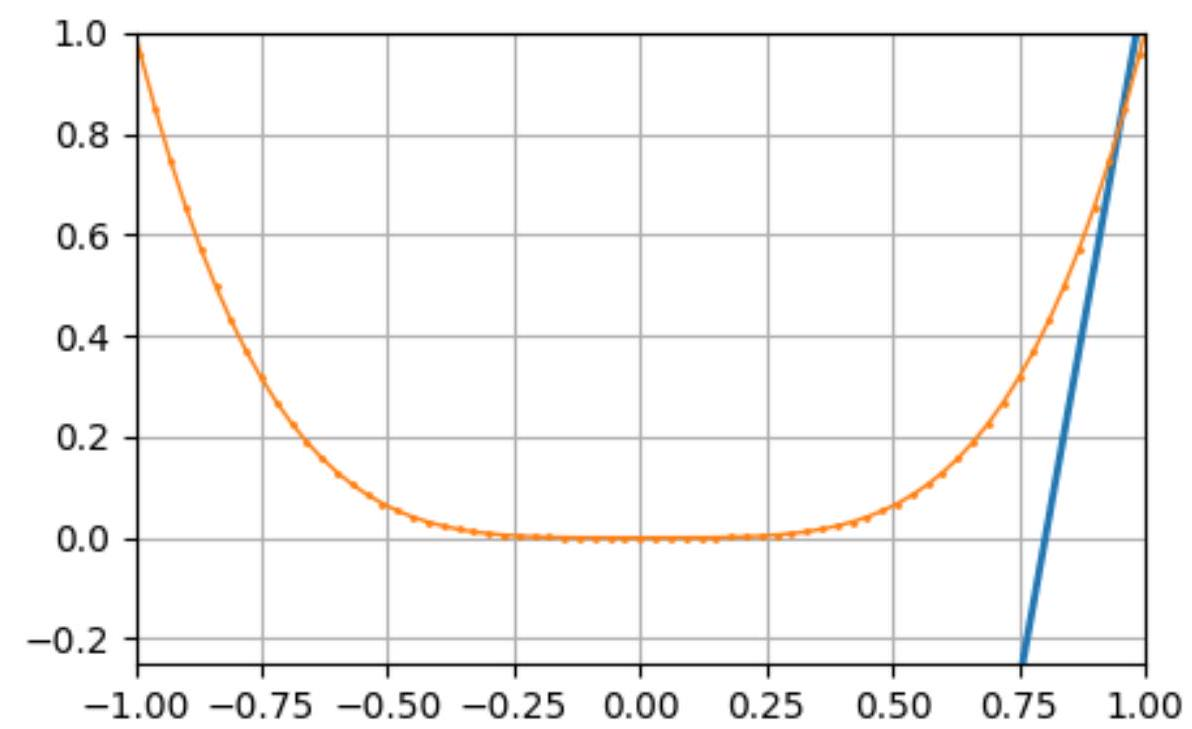
\includegraphics[max width=\textwidth]{2025_04_06_546e56f61867917283deg-2}
\end{center}

Newton's method visualization for $f(x)=x^{4}+.1$

\section*{Differentiation}
To find the derivative $f^{\prime \prime}\left(x_{n}\right)$ numerous algorithms can be used. The easiest to implement is finite differencing where

$$
f^{\prime \prime}(x) \approx \frac{\frac{f(x+h)-f(x)}{h}-\frac{f(x)-f(x-h)}{h}}{h}
$$

However, this becomes computationally expensive when $f^{\prime \prime}\left(x_{n}\right)$ is used numerous times across multiple $x_{n}$. A more difficult method to implement is Automatic Differentiation, where a tree is built containing the function and its derivatives, and is traversed multiple times at runtime. Computation of the derivative this way is more complex but is faster in higher order systems, as fewer matrix operations are required.

\section*{Method and complexity in Machine Learning}
In applications for machine learning, Newton's method optimization requires the following data: an initial guess for the minimum of the function, a tolerance level for convergence, and a maximum number of iterations. Here, the initial guess is randomly generated, but the further the guess is from the actual minimum, the longer it may take for Newton's method to find the minimum.

Newton's method converges to a solution at least quadratically (this holds only for the neighborhood of the root), in that each iteration the number of accurate digits approximately doubles. Nevertheless, this can be affected by a variety of factors. As mentioned in the previous paragraph, if the initial guess is very close to the solution, the number of iterations may be very few, but if it's very far, it may not only cause slow convergence, but even divergence and never find the minimum of the function. Additionally, Newton's method, because it's based on differentiation, relies on the function to have continuous first and second derivatives, so it is very inefficient or cannot be used at all if the function has discontinuities or singularities. Lastly, Newton's method ends when the change in the predicted solution is small enough or when the value of the prediction is very close to 0 . Newton's method's performance may also vary depending on the shape of the function. Functions with a relatively linear first derivative may have faster convergence in the input space, as the tangent line approximation of the first derivative by the second derivative is more accurate.

Because Newton's method has a quadratic convergence rate, it is considered to be a good choice based on the number of iterations needed to find the solution, however it can still have greater complexity than other optimization algorithms. This is mainly because each iteration requires calculating both the gradient (first derivative) and the Hessian (second derivative), so it can be very computationally expensive when used with a lot of variables. Also, the manipulation and storage of the Hessian matrix is very memory-expensive, especially for high dimensions. With $n$ variables, calculating the gradient is $O(n)$ and calculating the Hessian is $O\left(n^{2}\right)$. Lastly, solving the linear systems with any method is usually $O\left(n^{3}\right)$ when it's dense. The number of iterations can vary greatly, as it depends on the tolerance level, curvature of the function, and the initial guess.

\section*{Conclusion}
As we have not implemented these algorithms and benchmarked them against various types of problems, we do not know the efficiency of these algorithms yet.

\section*{Extensions and Applications}
Extensions include using Newton's method as the optimizer for other problems, such as physics engines, architecture design, or even other machine learning related applications not covered in our project (such as unsupervised or reinforcement learning). Other extensions include the use of other optimization algorithms for machine learning applications, perhaps most interestingly derivative-free algorithms (non-gradient based). For future work, if our findings suggest Newton's method can be useful, we could continue testing using larger networks and other frameworks. The applications of our work depend on the findings, but will all be related to machine learning.

\section*{References}
[1] "Newton's method," Wikipedia, \href{https://en.wikipedia.org/wiki/Newton%27s_method}{https://en.wikipedia.org/wiki/Newton's\_method} (accessed Mar. 7, 2025).\\[0pt]
[2] GeeksforGeeks, "Newton's method in machine learning," GeeksforGeeks, \href{https://www.geeksforgeeks.org/newtons-method-in-machine-learning/}{https://www.geeksforgeeks.org/newtons-method-in-machine-learning/} (accessed Mar. 7, 2025).\\[0pt]
[3] "Automatic differentiation," Wikipedia, \href{https://en.wikipedia.org/wiki/Automatic_differentiation}{https://en.wikipedia.org/wiki/Automatic\_differentiation} (accessed Mar. 7, 2025).


\end{document}
